\section{Resultater og målinger}
Dette afsnit indeholder alle målinger og resultater. 

\subsection{Skilz}
En samling af de kunstperler af evner \HM besidder i nuværende øjeblik.

\subsubsection{Mad kvalitet}
På figur \ref{fig:FoodBeer}\copyright \, ses vurderingen af madkvaliteten som funktion af alkoholindtag per dag i form af øl. Mængden af testpersoner er angivet til at være et sted mellem en halv til 60 personer grundet heftig sygdom\footnote{Alle uafhængige undersøgelse fraskriver enhver sammenhæng med mængden af sygdom og maden.} 

Bodeplottet viser tydeligt hvorledes \HM påvirkes af øl i løbet af dagen. Magnituden er normeret i forhold til en Noma kok, hvilket betyder $0dB$. Der ses en kraftig stigning i forhold til Noma kogen fra 1 øl og op efter. Omkring de 6-7 øl topper \HM med ca. 23 dB\footnote{Her noteres at 3dB er en fordobling af madkvalitet rent fysiks (subjektivt). Dog kræver det 10dB for at give en fordobling af madkvalitet rent psykologisk (objektivt).} Herefter falder madkvaliteten en squize for at falde på plads ved en konstant forstærkning på 14dB, dvs. mere end en fordobling af den psykologiske madkvalitet i forhold til Noma.
En vigtig lille detalje er at et bodeplot ikke kan vise 0 på Beers/day aksen hvilket er valgt, da tallet 0 aldrig fremkommer. 

Dog bør man notere sig faseskiftet \HM gennemgår i løbet af indtagelsen af øl gennem dagen. Dagen starter altid ud med at være forskudt $90 \deg$ grader, men falder ved omkring de 6-7 øl. Herover er madkvaliteten i fase.

Herpå kan der konkluderes at den optimale madkvalitet opnås som en finbalance mellem mad i topkvalitet og madkvalitet i fase.  

\begin{figure}[h!]
\centering
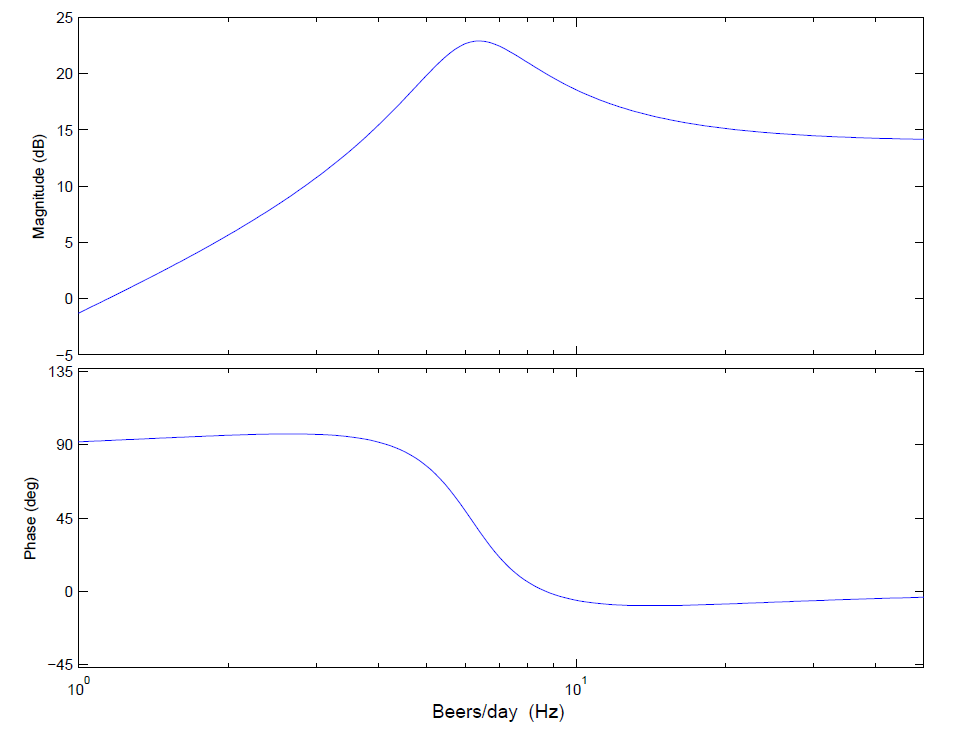
\includegraphics[width=0.8\columnwidth]{FoodQualityBeers.png}
\caption{Mad kvalitets vurdering som funktion af antal af øl indtaget per dag. 0 dB svarer til Noma kok.}
\label{fig:FoodBeer}
\end{figure}


\subsubsection{Succes (og det der hører til)}
Succes bliver ifølge standarden ISO666-69 opgivet efter antal bespiste personer og antallet heraf, som har været nødsaget til at lade livet grundet madforgiftning.\footnote{Antal personer, som har været nødsaget til at lade livet grundet madforgiftning, er fraregnet antal personer, som har været nødsaget til at lade livet grundet madforgiftning forsaget af dårlige råvarer. } 

På figur \ref{fig:ServeretPersonner}\copyright \,  er den akkumuleret antal af personer som \HM har serveret til. Der ses tydeligt en rivende udvikling fra 2009 frem til 2011. Der skal tages forbehold for at 2012 langt fra er overstået. En forecast af 2012 viser et skyhøjt antal bespiste personer på 750 ved udgangen af året ($\pm$ julefrokost, påskefrokost, andre hyggelige komsammener.)

\begin{figure}[h!]
\centering
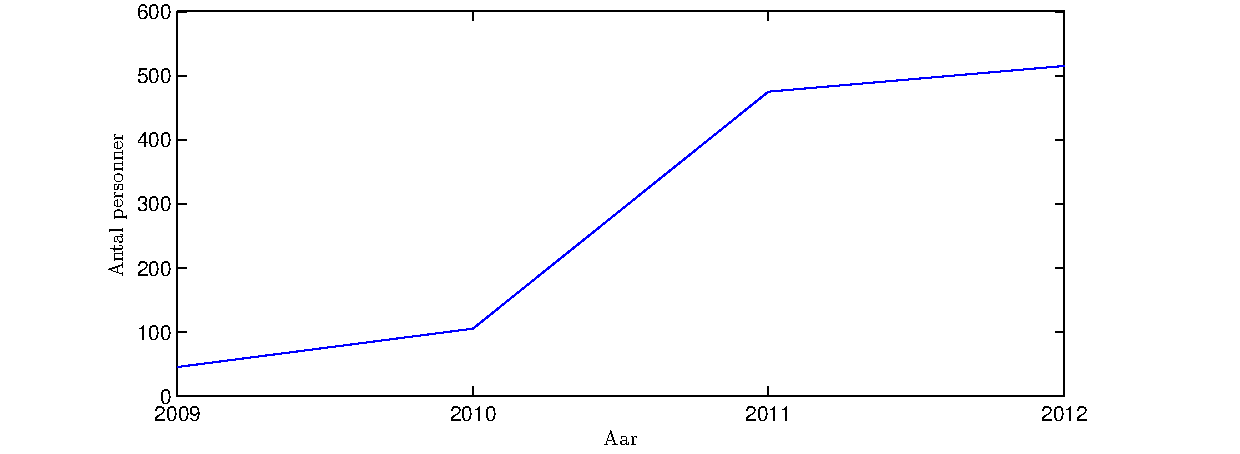
\includegraphics[width=0.8\columnwidth]{ServeretPersonner}
\caption{Akkumuleret serveret personer til dags dato.}
\label{fig:ServeretPersonner}
\end{figure}

På figur \ref{fig:DeadPeople}\copyright \, ses mængden af døde personer følge af servering af mad fra \HM. Grafen viser tydeligt mangel på udvikling indenfor dette område. Umiddelbart ville man have forventet en sinuskurve\footnote{Der er før vist en sammenhæng mellem mængden af døde og mængden af samlejer.}, men \HM formår at bibeholde en nulløsning. 

\begin{figure}[h!]
\centering
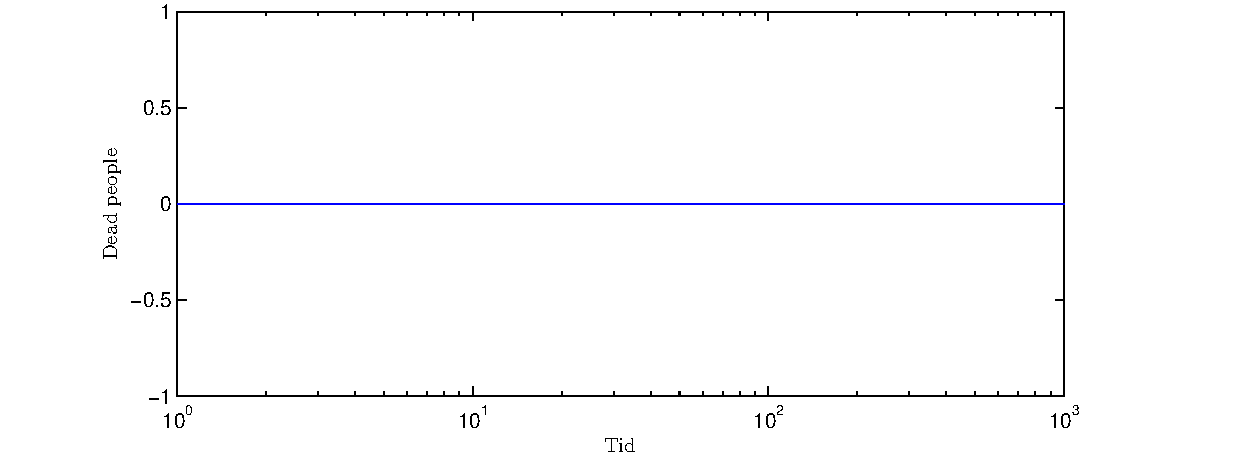
\includegraphics[width=0.8\columnwidth]{DeadPeople}
\caption{Antal af døde personer som funktion af serveringer.}
\label{fig:DeadPeople}
\end{figure}

\subsubsection{Ølbowling}
I løbet af årene har \HM udvist en stor interesse for den ædle sportsgren Ølbowling \cite{bib:url:BeerBow}. I tabel \ref{tab:BeerBow} vises de forskellige udfordrere gennem tiden med opgivelse af mængden af kampe, vundne, uafgjorte, tabte og antal point. 

Tabellen viser tydeligt et klart billede af et uovervindeligt hold, det 2100-århundredes champions, et rigtig vinderteam, plankebøf, super figther team of the century\cite{bib:url:2xThyboe}. Nogle medlemmer af Polyteknisk Forening har betvivlet denne optælling og beskyldt \HM for aftalt spil. Dog viser det sig ved en fintælling at den totale sum af point løber op, hvilket stemmer meget godt overens med 'Pænt Mange'.
\begin{table}[h!]
\centering
\begin{tabular}{|c|c|c|c|c|c|} \hline 
Modstander & Kampe & Vundne & Uafgjort & Tabte & Point \\ \hline \hline
Schlaikjer og forlovede & 4 & 4 & 0 & 0 & MAX \\ \hline
Vang og Nørr (Gamle B10) & 3 & 3 & 0 & 0 & MAX \\ \hline
RUC (til DSF konference) & 3 & 3 & 0 & 0 & MAX \\ \hline
Shus'ere & 4 & 5 & 0 & -1 & mere end MAX \\ \hline
Nørr og Fishcer (PF røvhuller) & 2 & 2 & 0 & 0 & MAX \\ \hline
Utallige russer & $\infty $ & $\infty - 1 $ & 0 & 1 & $\infty \cdot MAX -1$ \\ \hline \hline
Sum & $\infty + 16 $ & $\infty + 16$ & 0 & 0 & Pænt mange \\ \hline
\end{tabular}
\caption{Oversigt over ølbowlingskampe gennem tiderne for Holy \& Moly\texttrademark.}
\label{tab:BeerBow}
\end{table}

\subsubsection{Sovs}
Det er meget vigtig at der skelnes mellem sovs og sauce. \HM laver ikke saucer, kun sovse, og det er i rigelige mængder. Indtil videre er der to sovse ud af to, som har vist sig at have en rivende popularitet. Whiskeysovsen (grøn kurve) og Fernetsovsen\textregistered \copyright \texttrademark \, (blå kurve). Som der ses i figur \ref{fig:Sovse} har der op til i dag været en ganske nydelig popularitet men forecastet viser en tydelig stigning, både logaritmisk og eksponentielt. Whiskeysovsen har altid været værdsat som prikken over i'et blandt de bespiste personer til festmiddagen og specialt dagen derpå som supplement til brunch. Fernetsovsen\textregistered \copyright \texttrademark \, har oplevet en rivende udvikling\footnote{Særlig tak skal gives til PF-helten og Peter Tovte og venner.} de sidste år og der spås en lysende fremtid for denne specialitet, specielt i sydøst-asien. For at forbedre Fernetsovsen \textregistered \copyright \texttrademark \, er \HM ved at planlægge studietur til Milano for at snakke med Master of Fernet Branca folkene. 
\begin{figure}[h!]
\centering
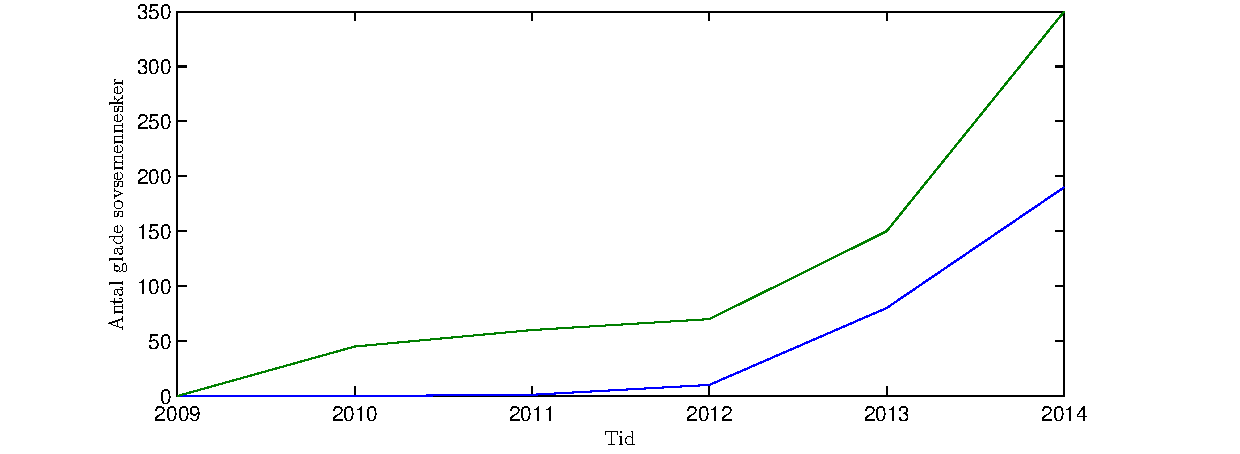
\includegraphics[width=0.8\columnwidth]{Sovse}
\caption{Popularitet af sovse - sofar inkl forecast.}
\label{fig:Sovse}
\end{figure}

\subsubsection{Rationelle løsninger}
En af de fantastiske skilz af \HM er deres rationelle løsningsmetoder. På figur \ref{fig:OlOvn} ses hvorledes temperaturen af øllet justeres fra 5 grader til 20 grader.\\

\begin{figure}[h]
\centering
\subfigure[Temperaturregulering af øl for at opnå optimal temperatur til ølbowling.]{
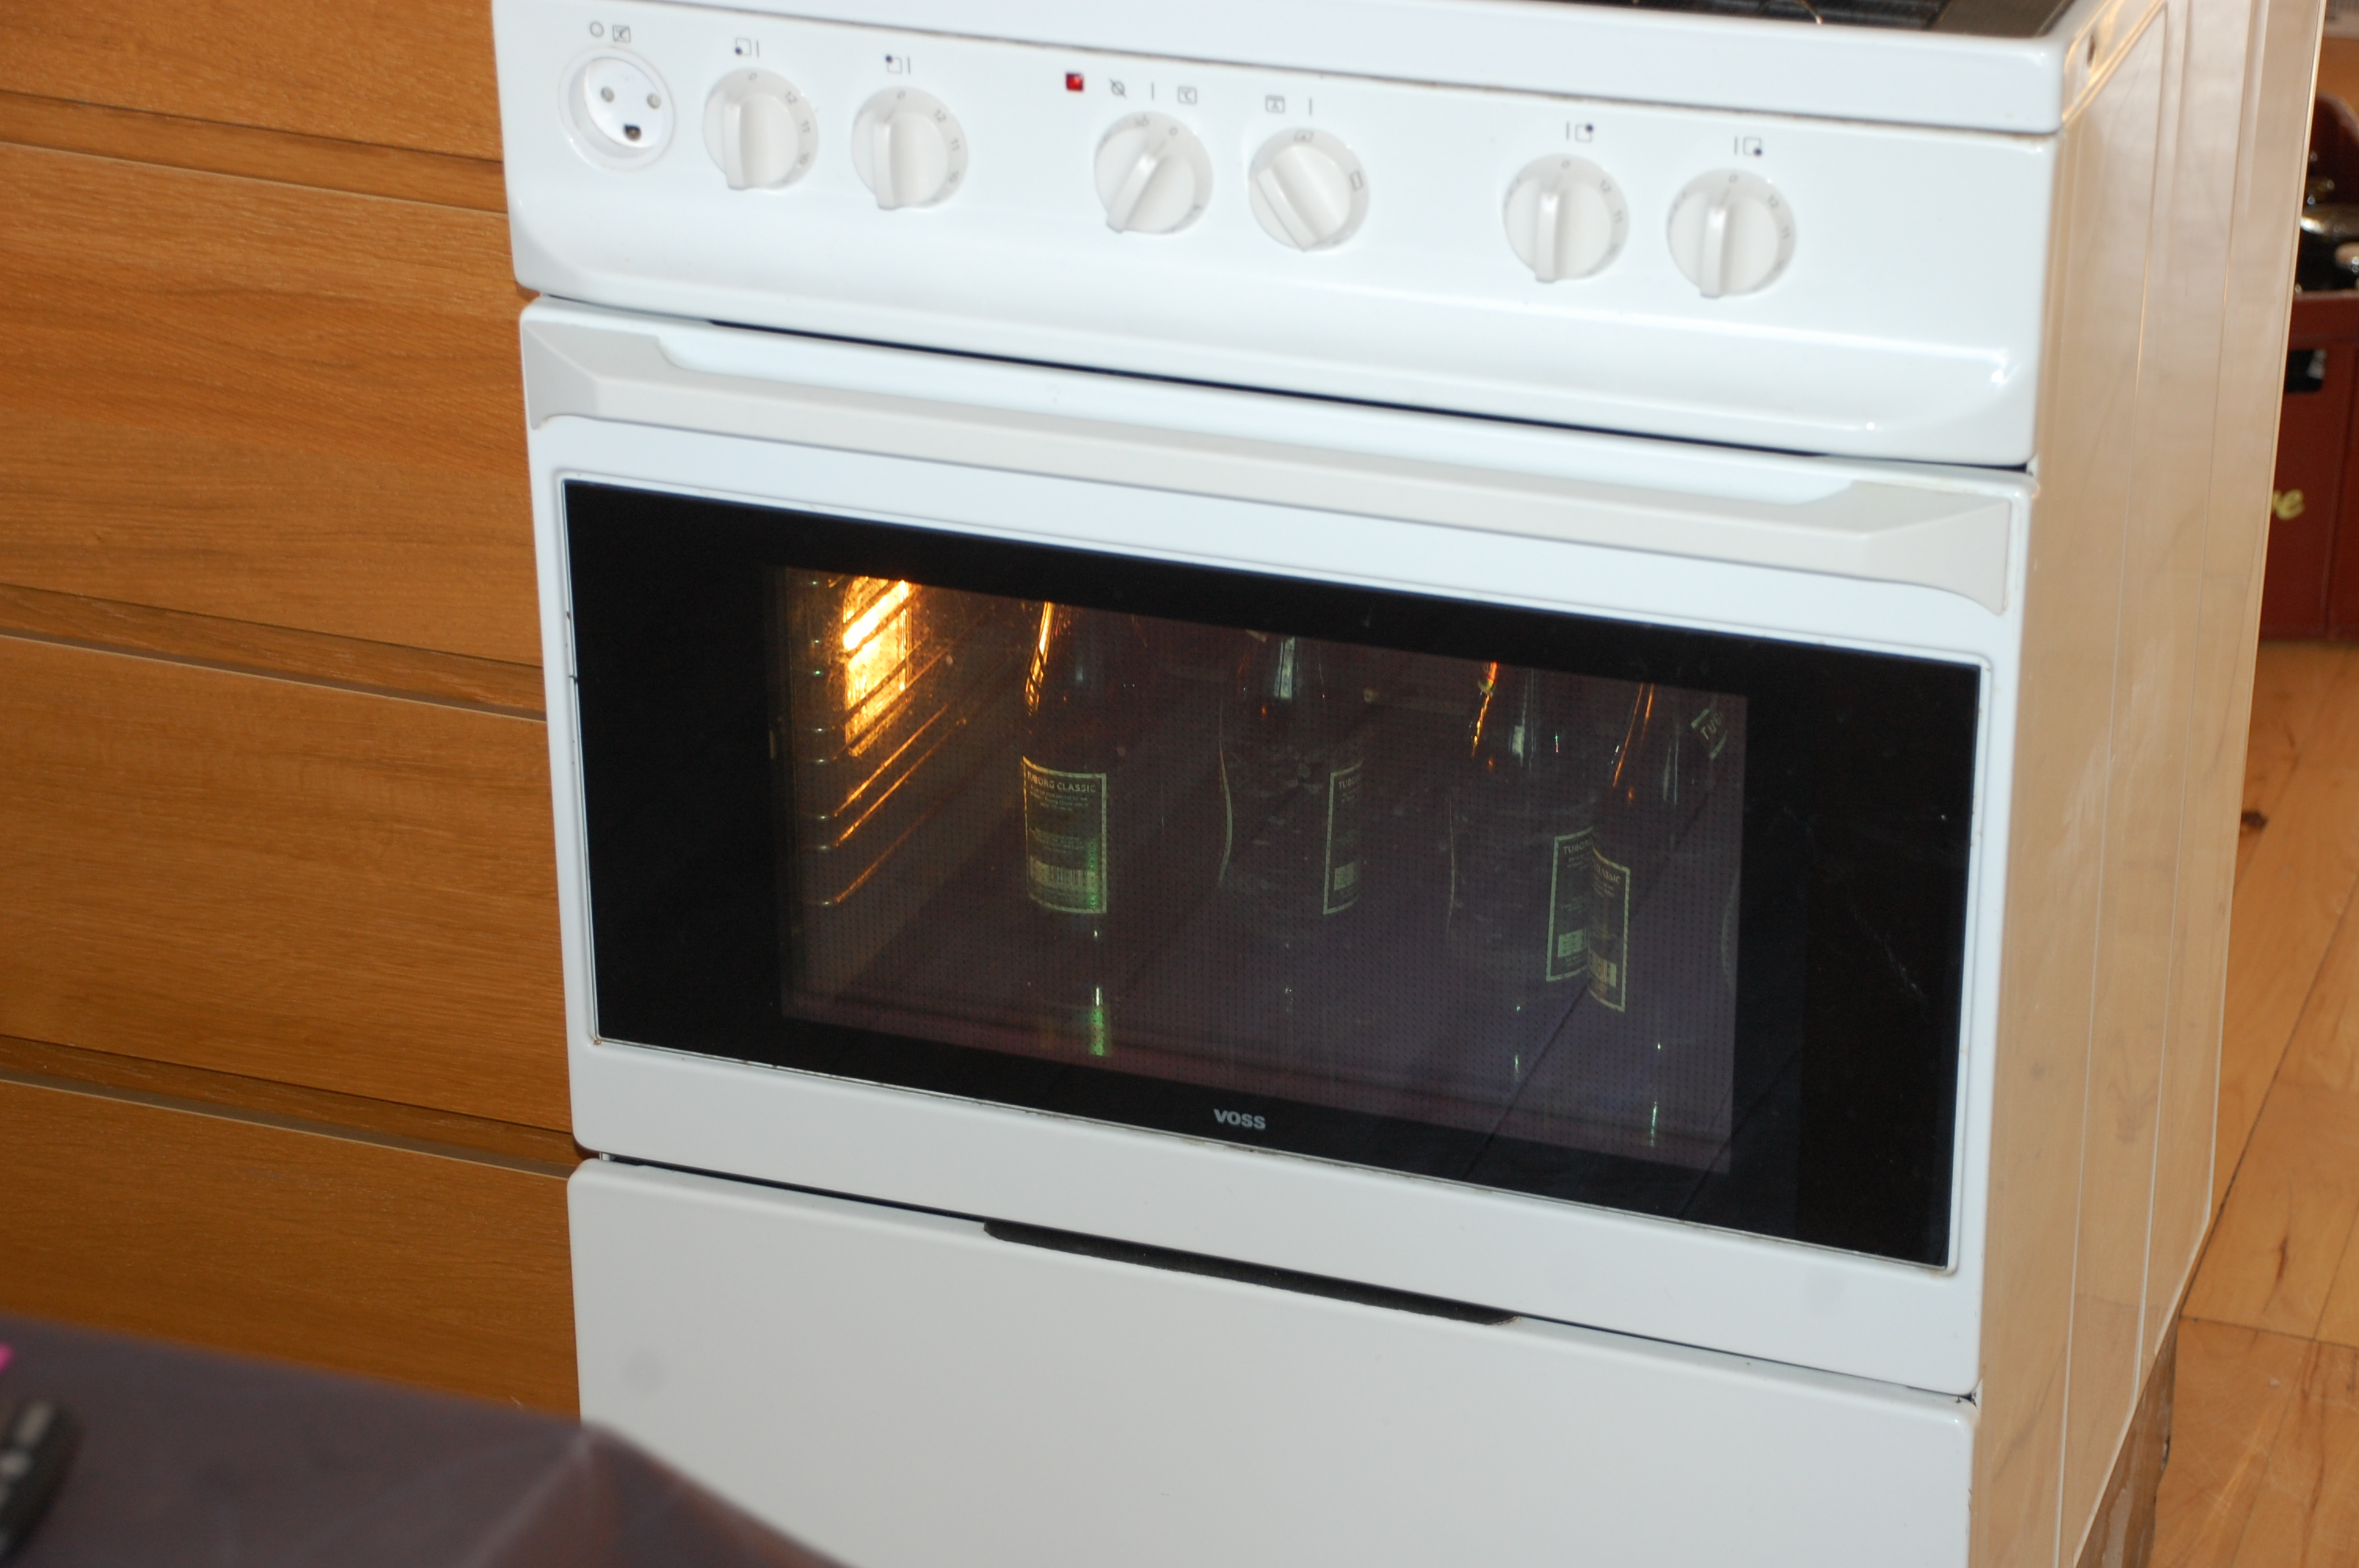
\includegraphics[width=0.45\columnwidth]{OlOvn}
\label{fig:OlOvn}
}
\subfigure[Solvognen version 0.1]{
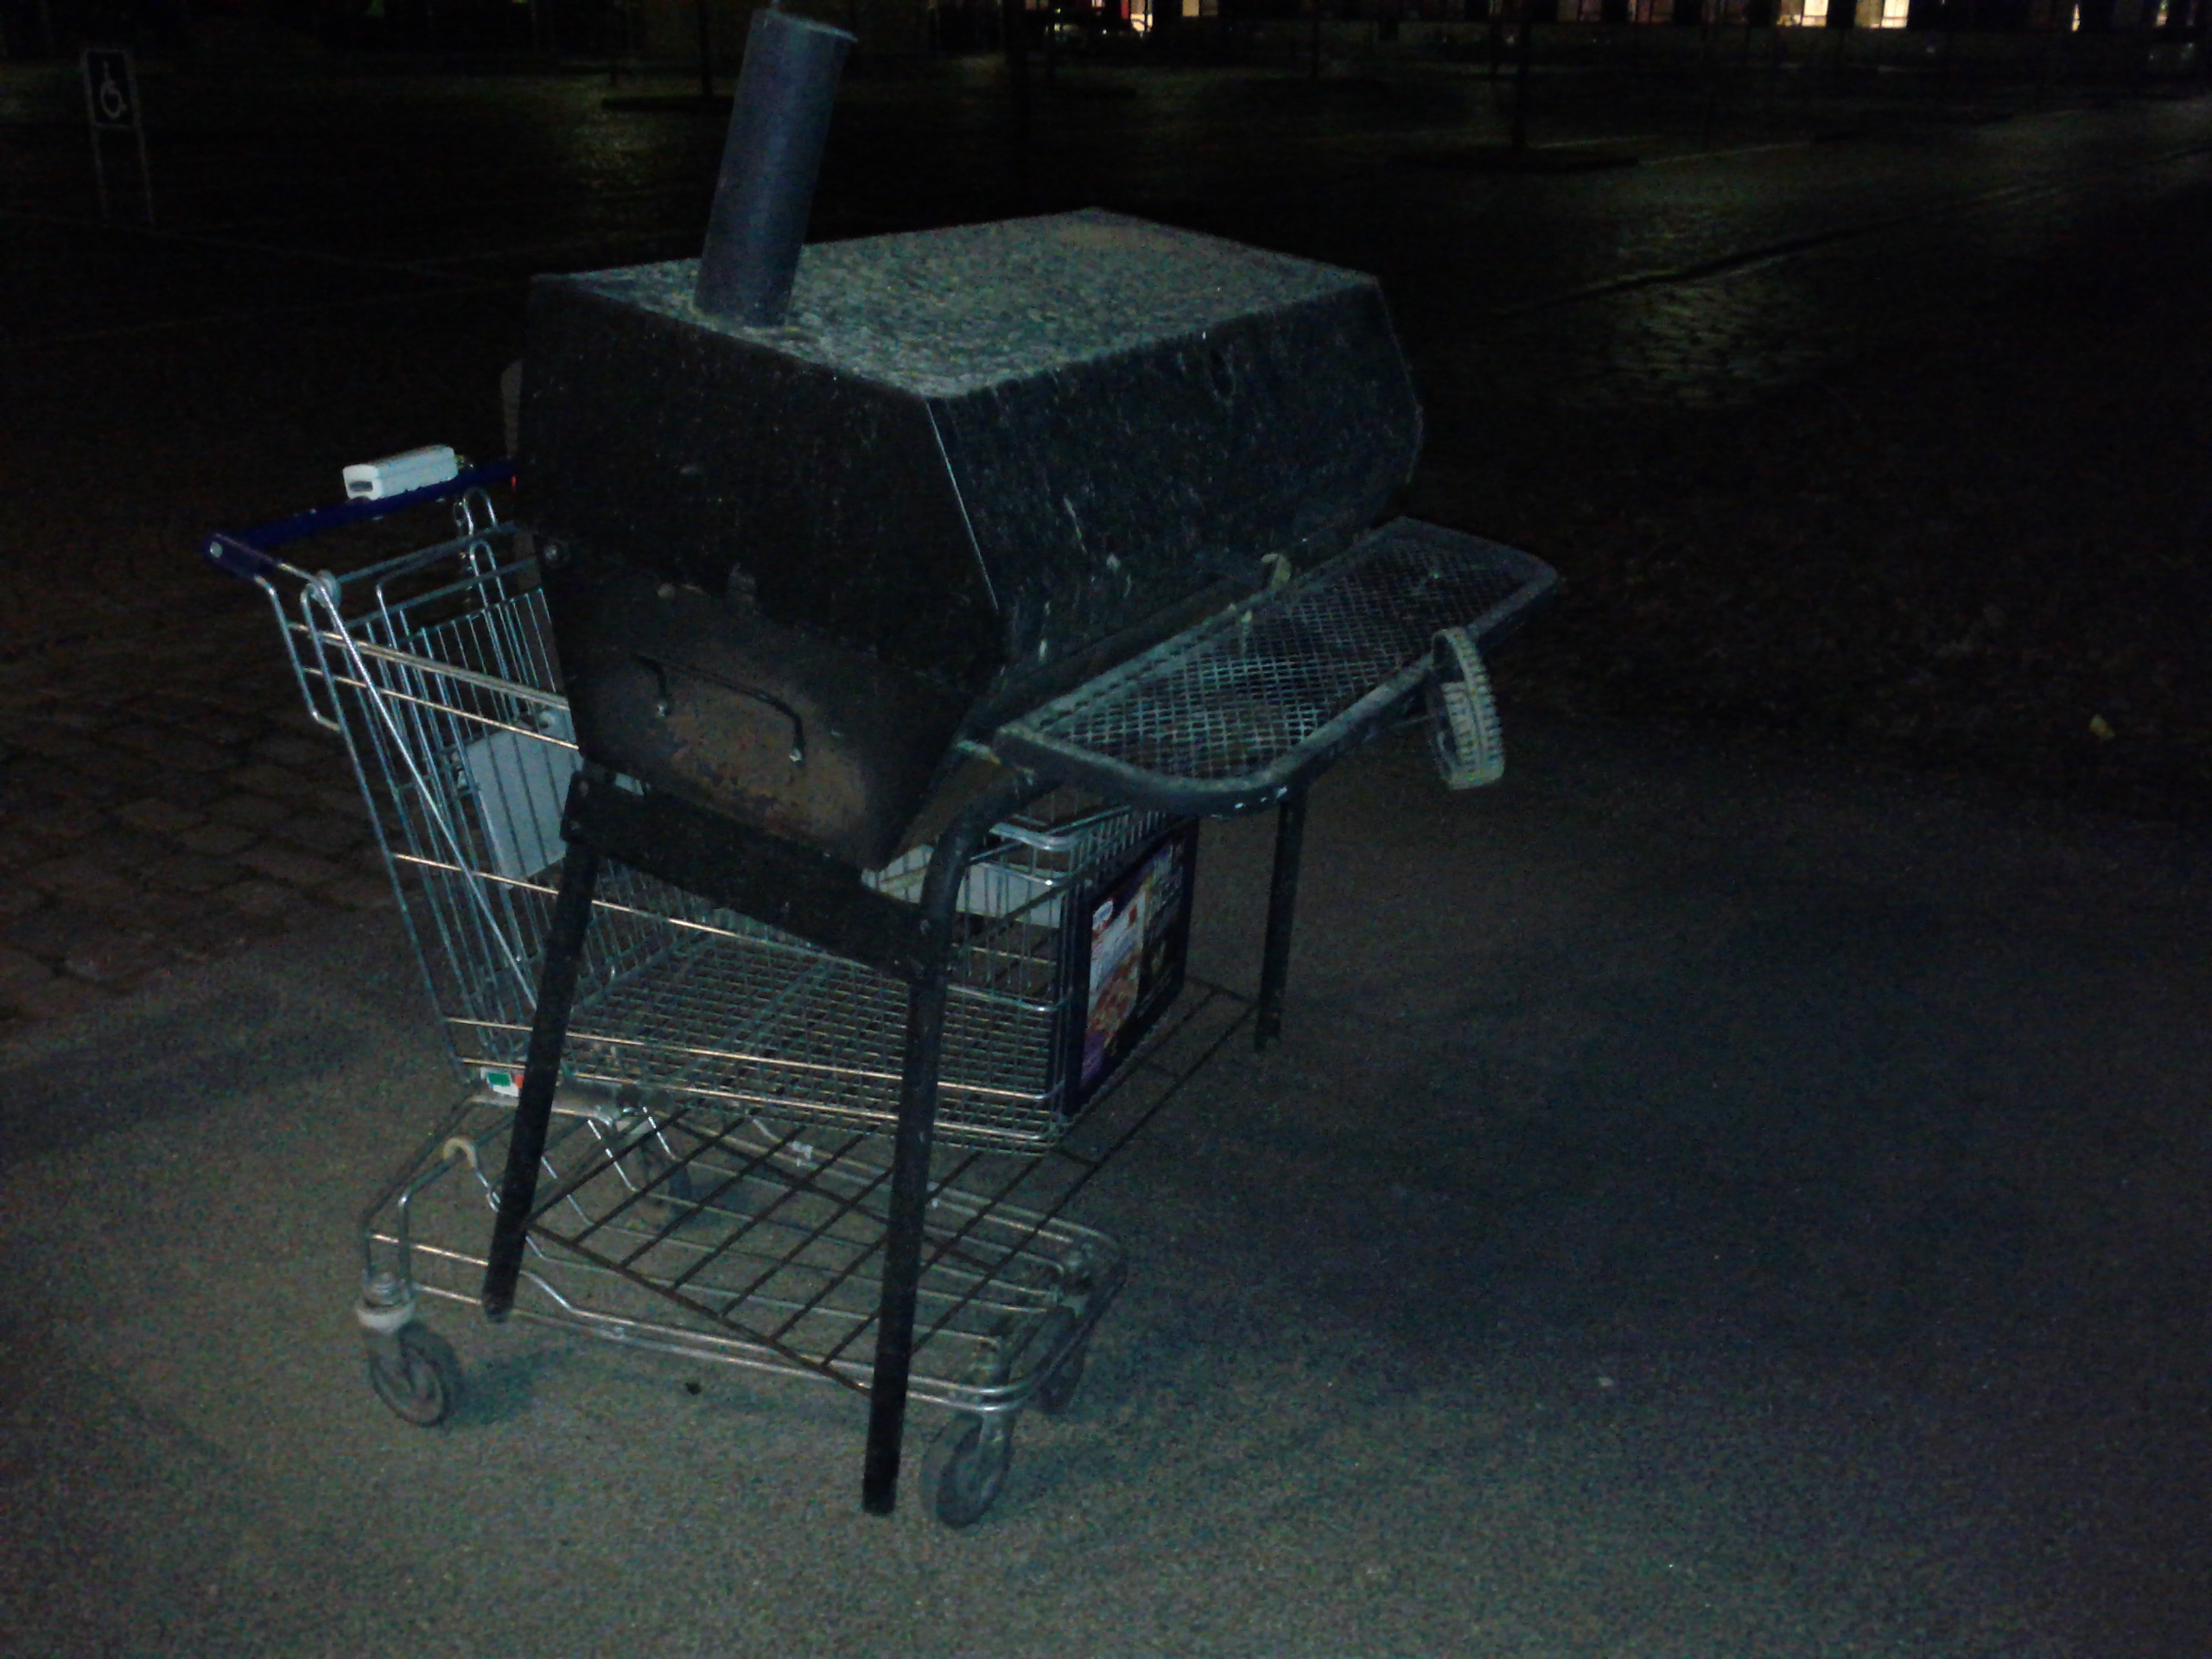
\includegraphics[width=0.45\columnwidth]{Solvogn2}
\label{fig:solvogn}
}
\caption{Rationelle løsninger}
\label{fig:rationelle}
\end{figure}

Det er velkendt at alle elsker grilmad, men ikke alle har en gril. Derfor har \HM arbejdet på projektet Solvognen og skabt version 0.1 som set på figur \ref{fig:solvogn}. Den muliggøre en kraftig stigning i mængden af grillbespiste personer og er oplagt som supplement til alverdens barrunder på DTU inklusiv motionsløbet.\\

\subsection{Bemærkelsesværdige madbedrifter}
Gennem tiden har \HM præsteret et væld af helt igennem fantastiske og særdeles bemærkelsesværdige madbedrifter. For ikke at gøre denne rapport lang vil der kun blive nævnt et mindre udpluk her.\\

\subsubsection{Mad til 45 mennesker på 45 minutter}
En torsdag aften op til Fællesrådsmøde i Polyteknisk Forening formåede Holy fra \HM desværre at glemme at han var ansvarlig for mad til mødet. Dette blev ham påpeget 45 minutter før maden skulle være færdig. Han skyndte sig hurtigt at slå pjalterne sammen med Moly fra \HM, hvorefter de gik i madlavnings-"mode". De skyndte sig over i Netto for at købe mad til de 45 mennesker som stod på til at spise. Deres første ide var at lave pita brød, men da Netto kun lå inde med 1 pakke faldt moralen drastisk. Dog kun for en stund. Sekundet efter fik \HM ideen at servere mexikanske pandekager. Der blev hurtigt handlet ind og samtidig begyndte de over telefon at koordinere en produktionslinje oppe i PF køkkenet.

Ved ankomsten til PF køkkenet stod køkkenassistenterne klar med speciel fremstillet produktionslinje til at skære grøntsager og stege kød. Selvom der der var travlt i køkkenet mistede \HM på intet tidspunkt overblikket og troen på at maden ville være klar til tiden. Og som de havde forventet, så kunne de første sætte sig til bords klokken 17:00 og spise som forventet. Alle var glade, ingen døde, maden var klar til tiden, alt i alt, en spektakulær bedrift af \HM.

\subsubsection{\HM Pandekager}
\HM har, som enhver kok med respekt for sig selv, opfundet deres egne retter. Her kan blandt andet nævnes Fernetsovsen\textregistered \copyright \texttrademark \ og \HM Panderkager. Fernetsovsen\textregistered \copyright \texttrademark \ er en forretningshemmelighed men tilgengæld er de berømte \HM Panderkager et open source madprodukt.

\begin{figure}[h!]
\centering
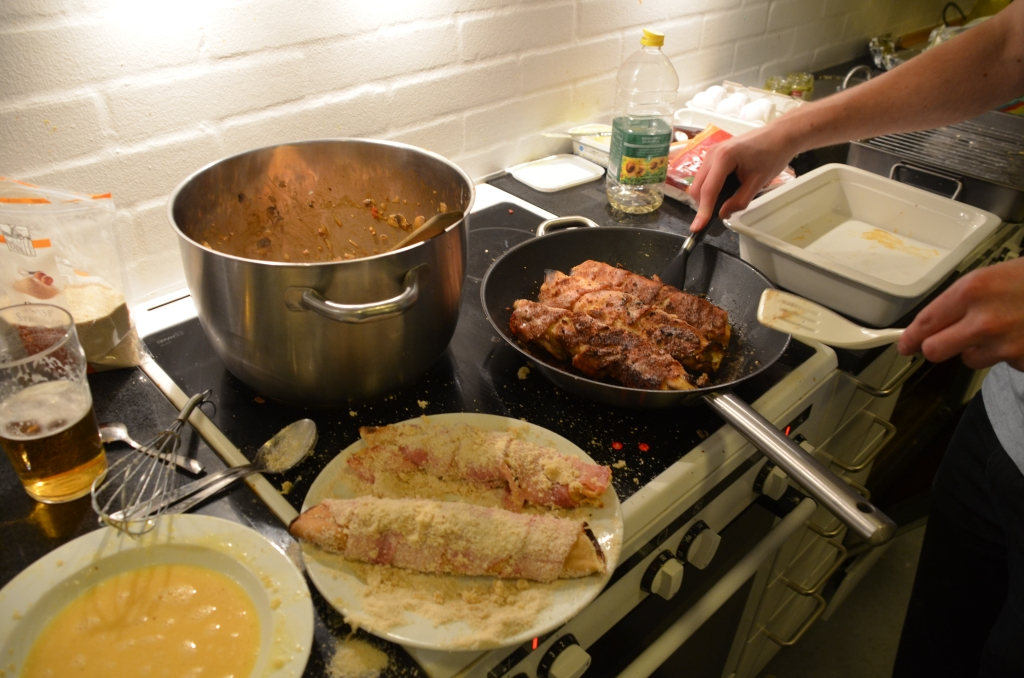
\includegraphics[width=0.8\columnwidth]{/KABSmad/12}
\caption{Produktion af \HM Pandekager.}
\label{fig:pandekager}
\end{figure}

Ideen til \HM Panderkagerne opstod på baggrund af eksperimenter med bacon og panering. Derefter blev PF køkkenet reserveret og KABS 12 "ansat" som testpersoner. På selve dagen startede \HM ud med et eventyr i form af en HC Andersen øl for at sikre madkvaliteten i henhold til figur \ref{fig:FoodBeer}. Derefter blev en dejlig pandekagedej bikset sammen med øl som special ingrediens samtidig med at en god omgang oksekød med ost og salsasovs blev kokkereret. 

Næste skridt var at opsætte produktionslinjen som vist i figur \ref{fig:pandekager}. Først en pande til at lave pandekagerne. Så over på en tallerken hvor fyldet blev puttet i og pandekagen rullet. Dernæst wrappet med baconskiver og sat ind i ovnen på 200 grader i 5 minutter. Dernæst blev de rullet i æg og rasp og til sidst over på panden, hvor de blev paneret i rigeligt smør.

Reaktionerne fra testpersonerne var pure positive. Billeder fra forsøget kan ses i appendix \ref{app:kabsmad}. 

\subsection{H\&M-ruten i Østdanmark eksl. Bornholm og resten af Sverige.}
På figur \ref{fig:Kort} ses den højt anerkendte H\&M-rute som for nylig har oversteget Marguerite-ruten som den mest besøgte\cite{bib:url:Marguerit}. Turen er optimeret til at give et godt supplement af de tre basale samfundssøjler: natur, kultur og øl\footnote{Ikke ses som konkurrence blandt de tre søjler, men mere som et solidt fundament.} Den kvikke Housetrip planlægger vil notere sig hvorledes at ruten omfatter samtlige rusture 2010 $\pm$. Deraf konkluderes at alt er besøgt, intet er tabt, intet er vundet, det hele er som det var før, alle er glade.  

\begin{figure}[h!]
\centering
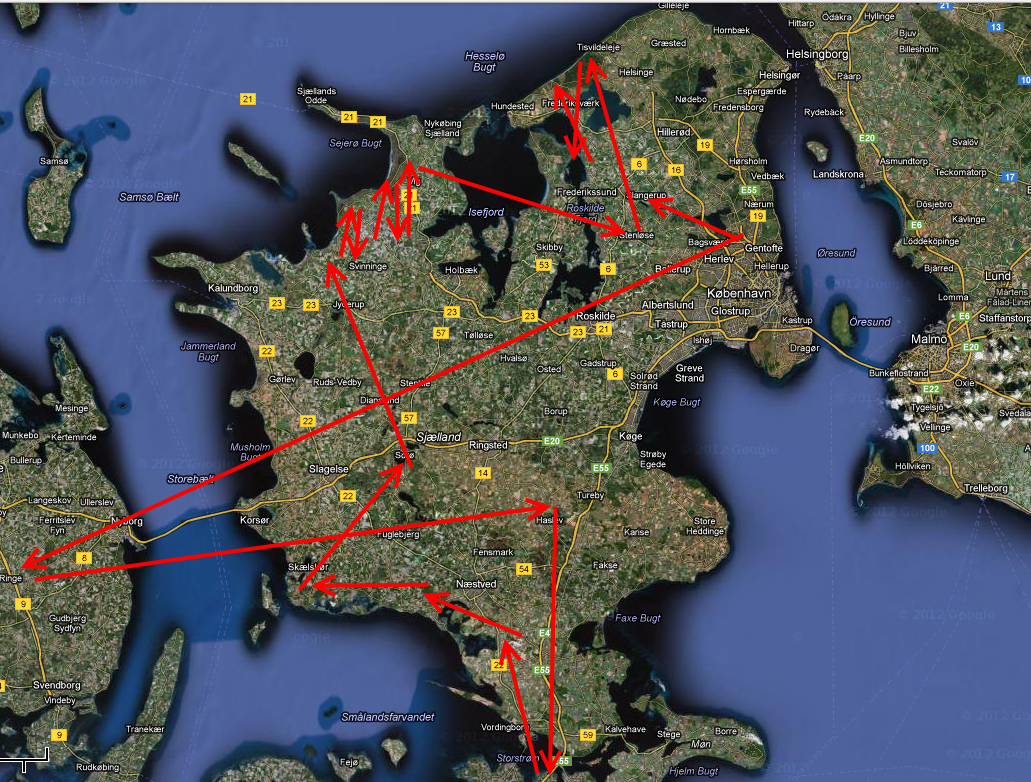
\includegraphics[width=\columnwidth]{Kort}
\caption{Margueritruten - steder hvor \HM har serveret fadøl til STOR glæde for den almene rus.}
\label{fig:Kort}
\end{figure}